\chapter{Particle Filter}
\label{chp:partFilter}
A particle filter is a method of estimating and describing the state of a system, as a set of samples of a posterior belief.
In the context of a particle filter, each sample is called a particle, which is a concrete instance of the system state, i.e. a hypothesis as to how the real world state might be.
Since the filter represents a distribution by a set of particles, instead of a parametric form such as a Gaussian, we can consider a particle filter to be non parametric.



%!TEX root = ../../report.tex

\begin{figure}[!b]
    \centering
    
    % Setup box for subfigure
    \subcaptionbox[Short Subcaption] 
        % Subcaption and label for subfigure
        {Initial state of a particle filter. The particles are randomly spread throughout the entire map and the best guess of the robot position is a random ''cluster'' of particles. \label{subfig:demo1}}
        % Size of figure and subcaption width
        [0.45\textwidth]
        % Figure to include (width should match the above width
        {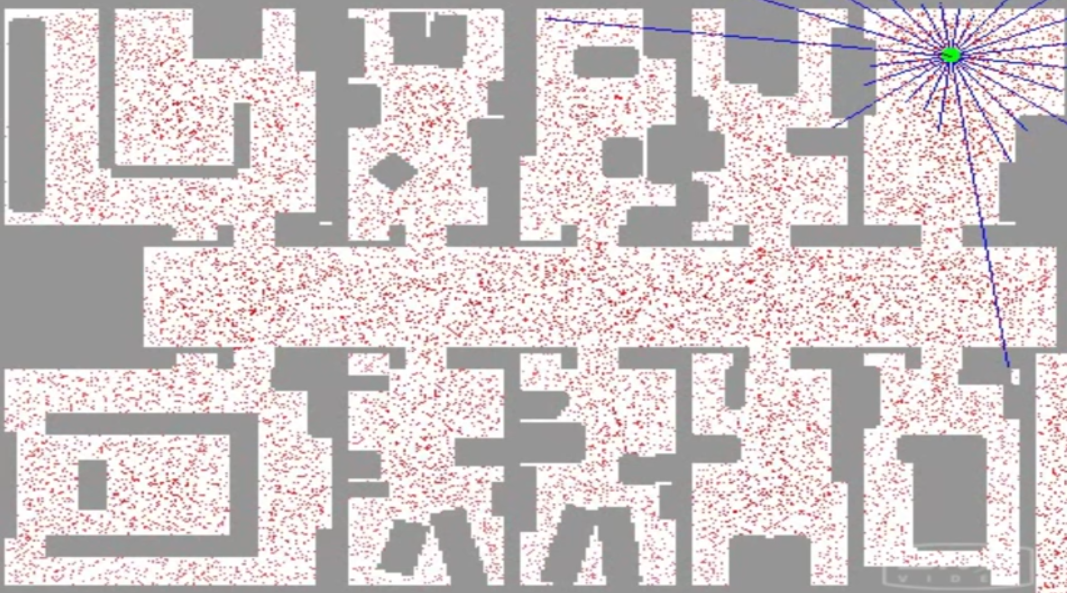
\includegraphics[width=0.45\textwidth]{ParticleFilter/demo1.png}}
%
\hspace{0.02\textwidth} % Seperation
%
    % Setup box for subfigure
    \subcaptionbox[Short Subcaption]
        % Subcaption and label for subfigure
        {After a few measurements, movements and resamples we begin to see a few particle clusters forming. The robot now believes that it is located in the corridor, but is still not quite sure where exactly. \label{subfig:demo2}}
        % Size of figure and subcaption width
        [0.45\textwidth]
        % Figure to include (width should match the above width
        {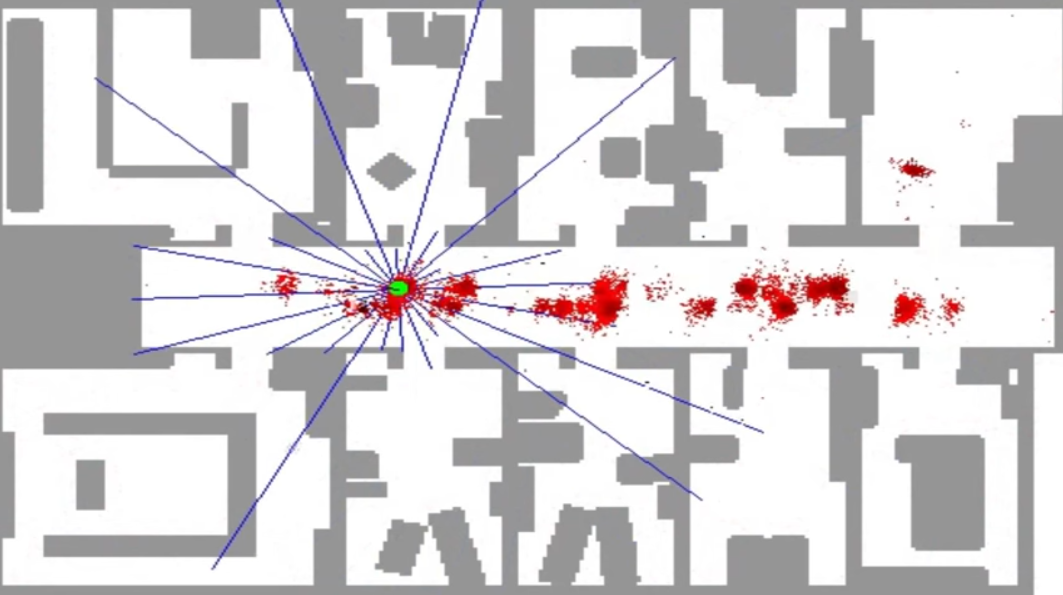
\includegraphics[width=0.45\textwidth]{ParticleFilter/demo3.png}}%
%
\\ % Seperation
%
    % Setup box for subfigure
    \subcaptionbox[Short Subcaption]
        % Subcaption and label for subfigure
        {As the robot continuously measure, move and resample it narrows down the possible positions. Here we see two particle clusters with quite strong beliefs, but the robot is still unable to tell exactly which cluster is the right one, due to the symmetry of the corridor.\label{subfig:demo3}}
        % Size of figure and subcaption width
        [0.45\textwidth]
        % Figure to include (width should match the above width
        {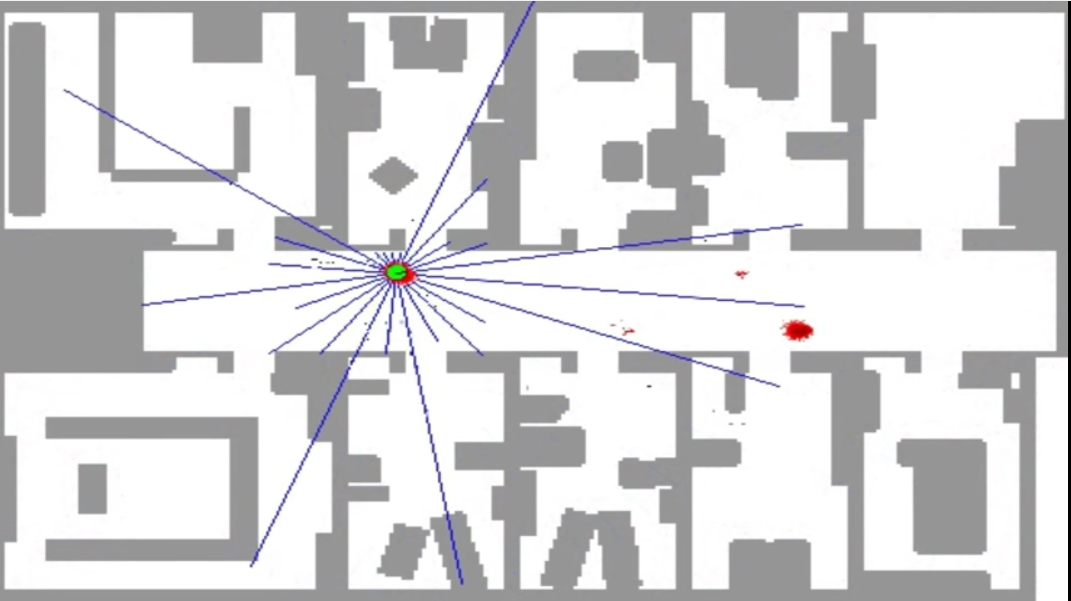
\includegraphics[width=0.45\textwidth]{ParticleFilter/demo4.png}}
%
\hspace{0.02\textwidth} % Seperation
%
    % Setup box for subfigure
    \subcaptionbox[Short Subcaption]
        % Subcaption and label for subfigure
        {When to robot enters a room, it is able to differentiate the rooms from each other and thus eliminate the incorrect belief of the other particle cluster, ending up with one good approximation to the actual position in the map. \label{subfig:demo4}}
        % Size of figure and subcaption width
        [0.45\textwidth]
        % Figure to include (width should match the above width
        {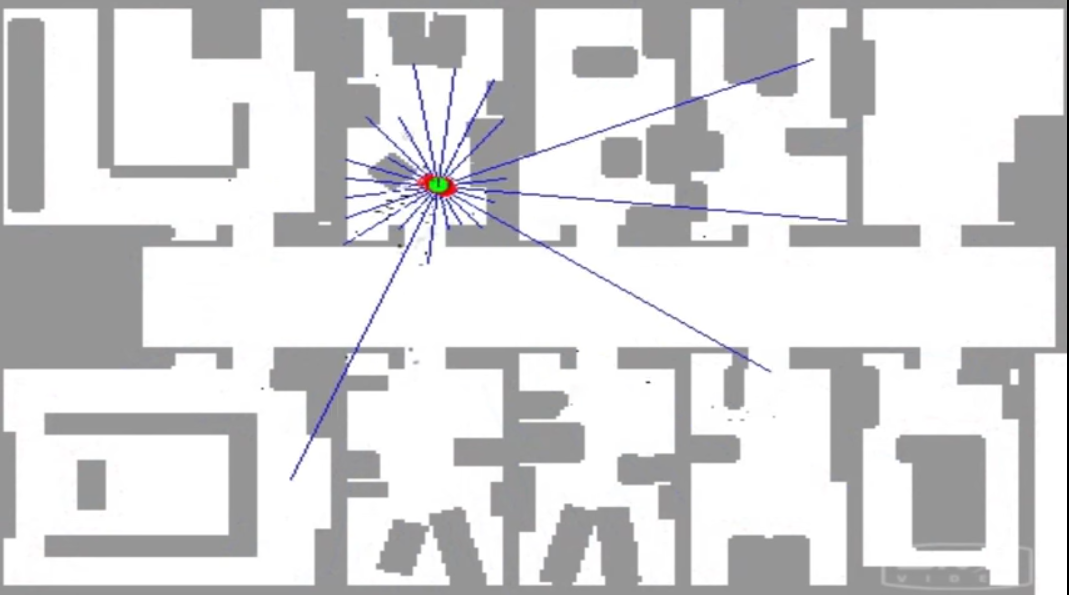
\includegraphics[width=0.45\textwidth]{ParticleFilter/demo5.png}}

    % Caption and label of whole figure set
    \caption[Short Caption]{Illustration of global localization using a particle filter. The map is a corridor and multiple rooms, where the white areas are accessible and the grey areas are walls, furniture etc. Each red dot represents a particle and the green circle represents the best guess of the robots position at each specific time.}
    \label{fig:particleDemo}
\end{figure}


The state estimations of particle filters are in practice applied to robotics in form of global localization.
Global localization means that a robot with an unknown position, in an otherwise known map, can identify its approximate position through a series of sensor measurements and controlled movements.

The principle of using a particle filter for global localization is best explained through an illustrative example. 
Figure \ref{fig:particleDemo} shows 4 stages og the state estimation, where figure \ref{subfig:demo1} show the initial state, where we know nothing about the robots actual position and therefore spread particles all over the map.
As the robot measures e.g. distances to different objects and moves around, we learn more about the position and can eliminate all the particles that doesn't fit our new beliefs, which in figure \ref{subfig:demo3} leads to two clusters of particles.
The two clusters are our best estimates due to the symmetry of the corridor, and the robot therefore has to move into one of the distinguishable rooms to identify the correct cluster, as shown in figure \ref{subfig:demo4}.

The filter actually builds on the \emph{survival of the fittest} thought, where the particles that best fit into the context of the robots measurements and movements are kept and copied, while particles that fits poorly are eliminated.
How well each particle fits the measured pose is expressed through importance weights, $w$, which are used in the algorithm of a particle filter to chose which particles to keep and which to eliminate.

The algorithm is recursive, i.e. the belief $bel(x_t)$ is constructed from the previous belief $bel(x_{t-1})$, that existed one time step earlier. 
Therefor the set of particles $X_{t-1}$ is one of the inputs to the algorithms.
The other inputs are the new measurement $z_t$ and the most recent set of movements controls $u_t$.
The basic form of the particle filter algorithm is listed in table \ref{tab:partAlgo}.
Line 4-5 moves a particle $x_{t-1}^{[n]}$ to $x_t^{[n]}$ based on the control sequence $u_t$ and assigns a new importance weight, $w_t^{[n]}$ according to the measurement $z_t$.\\
This new importance weight is then used in line 8-11 to determine which particles to keep and which to eliminate in order to generate the new belief, represented be a set of particles, $X_t$.
A process also known as resampling.

\begin{table}[!b]
    \caption[Short Caption]{The basic particle filter algorithm.}
    \label{tab:partAlgo}
\begin{tabular}{|l p{12cm}|}
    
    \hline
    1: \qquad  & \textbf{Algorithm Particle\_ filter}($X_{t-1}, u_t, z_t$)\textbf{:} \\
    2: \qquad  & \qquad $\bar{X_t} = X_t = Ø$ \\
    3: \qquad  & \qquad for $n = 1$ to $N$ do\\
    4: \qquad  & \qquad \qquad sample $x_t^{[n]} \sim p(x_t | u_t, x_{t-1}^{[n]})$\\
    5: \qquad  & \qquad \qquad $w_t^{[n]}=p(z_t|x_t^{[n]}$\\
    6: \qquad  & \qquad \qquad $\bar{X_t} = \bar{X_t} + \langle x_t^{[n]}, w_t^{[n]} \rangle $  \\
    7: \qquad  & \qquad endfor \\
    8: \qquad  & \qquad  for $n = 1$ to $N$ do\\
    9: \qquad  & \qquad \qquad draw $i$ with probability $\propto w_t^{[i]}$\\
    10: \qquad & \qquad \qquad add $x_t^{[i]}$ to $X_t$\\
    11: \qquad & \qquad endfor\\
    12: \qquad & \qquad return $X_t$\\
    \hline
\end{tabular}
\end{table}

\noindent The resampling process is the part of the algorithm where the particles should converges towards the robots true position.
But the process of choosing which particles to keep and which to kill is not trivial and can be approached in multiple ways, one of which is called \emph{Low Variance Resampling} algorithm.

The Low Variance Resampling algorithm is a probabilistic approach, where the particles to survive is chosen from a probability distribution based on each particles weight.
%This probability is introduced by the use of a random variable called $\beta$.
%\begin{align*}
%    \beta = 2 \cdot w_{max} \cdot U(0, 1)
%\end{align*}
%The $\beta$-value is a step size in a cyclic environment of the particle weights as shown i figure \ref{fig:RePart}. 
%Each particle is scaled by its weights and if you step twice in a row in the same particle, this particle is kept for the next iteration of the particle filter.
The steps of the Low Variance Resampling algorithm is as follows:
\begin{enumerate}
    \item Chose an initial index, $i$ from a uniform distribution of all particles in the set to be resampled, $i=U(1,N_{particles})$
    \item Generate a new random $\beta$-value, $\beta = 2 \cdot w_{max} \cdot U(0, 1)$
    \item if $\beta > w_t^{[i]}$
    \begin{enumerate}
        \item Subtract the weight from $\beta$.
        \item Increment the index $i$.
    \end{enumerate}
    \item if $\beta < w_t^{[i]}$
    \begin{enumerate}
        \item Add the particle to the new set of particles, $X_{t+1}$
    \end{enumerate}
    \item Repeat from step 2, until $sizeof \left( X_{t+1} \right) = sizeof \left( X_{t} \right)$
\end{enumerate}















